\begin{frame}
	\frametitle{Atmosphäre - Luftmassen}

	\begin{figure}
		\centering
		\begin{tikzpicture}
			\node (image1) {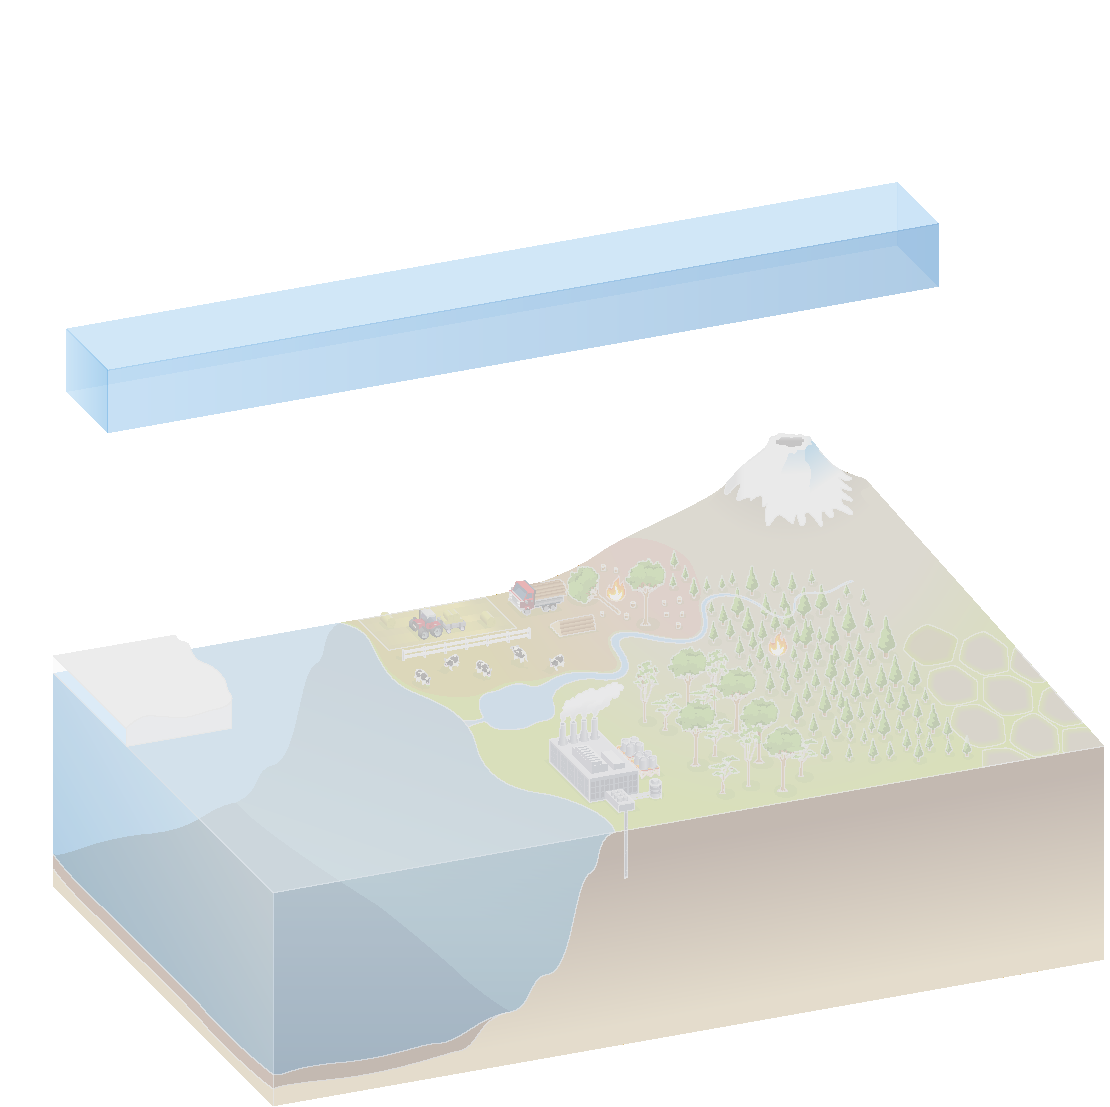
\includegraphics[trim={1cm 0cm 0cm 3cm}, clip, width=0.55\linewidth]{%
        	bilder/climate_components/global_climate_components_atmosphere.pdf}};
			\onslide<2|handout:0>\node (image2) at (image1.east) [xshift=-0.9cm]{%
					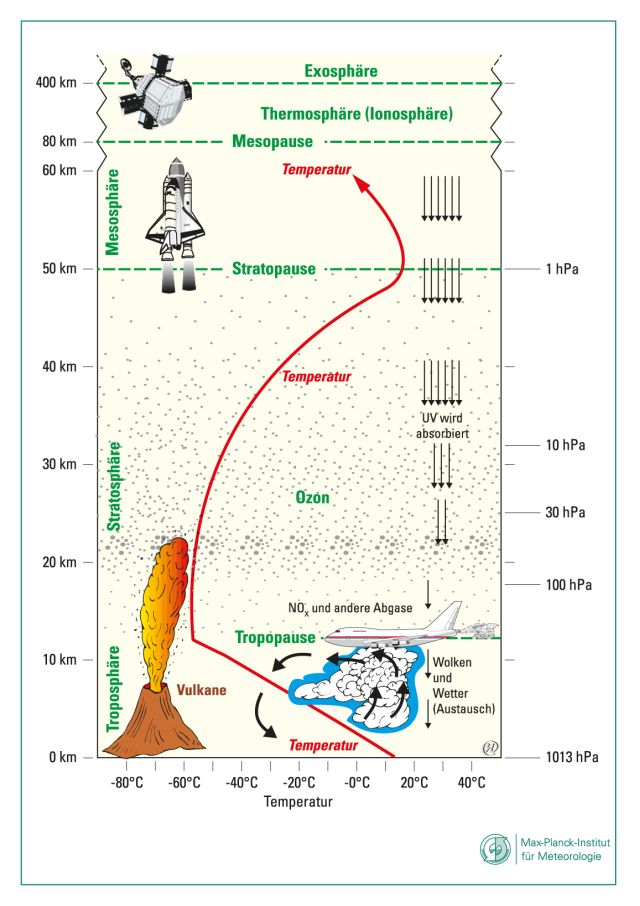
\includegraphics[width=0.35\linewidth] der Atmosphärenmasse, enthält fast allen Wasserdampf
			    \item[] Hier finden alle wetterrelevanten Phänomene statt
			  \end{itemize}
			  \item Stratosphäre, \SIrange{12}{50}{km}, \SIrange{-60}{0}{\celsius}, Ozon sorgt für Temperaturanstieg durch UV-Absorption
			  \item Mesosphäre, \SIrange{50}{80}{km}, \SIrange{-100}{0}{\celsius}, Temperatur fällt
			  \item Thermosphäre, \SIrange{80}{400}{km}, extrem geringe Teilchendichte, daher Temperatur nicht bestimmbar, Weltraum
			  \item Exosphäre, \SIrange{400}{1000}{km}, quasi Vakuum
			\end{itemize}
			\item[] Passt sich am schnellsten an Änderungen an
			\item[] in der planetaren Grenzschicht (\SIrange{1}{2.5}{km}): Reibung wichtig $\rightarrow$ starke vertikale Unterschiede in diesem Bereich der Atmosphäre
		\end{itemize}
		}
\end{frame}

\begin{frame}
	\frametitle{Globale Atmosphärische Zirkulation}

	\begin{figure}
		\centering
		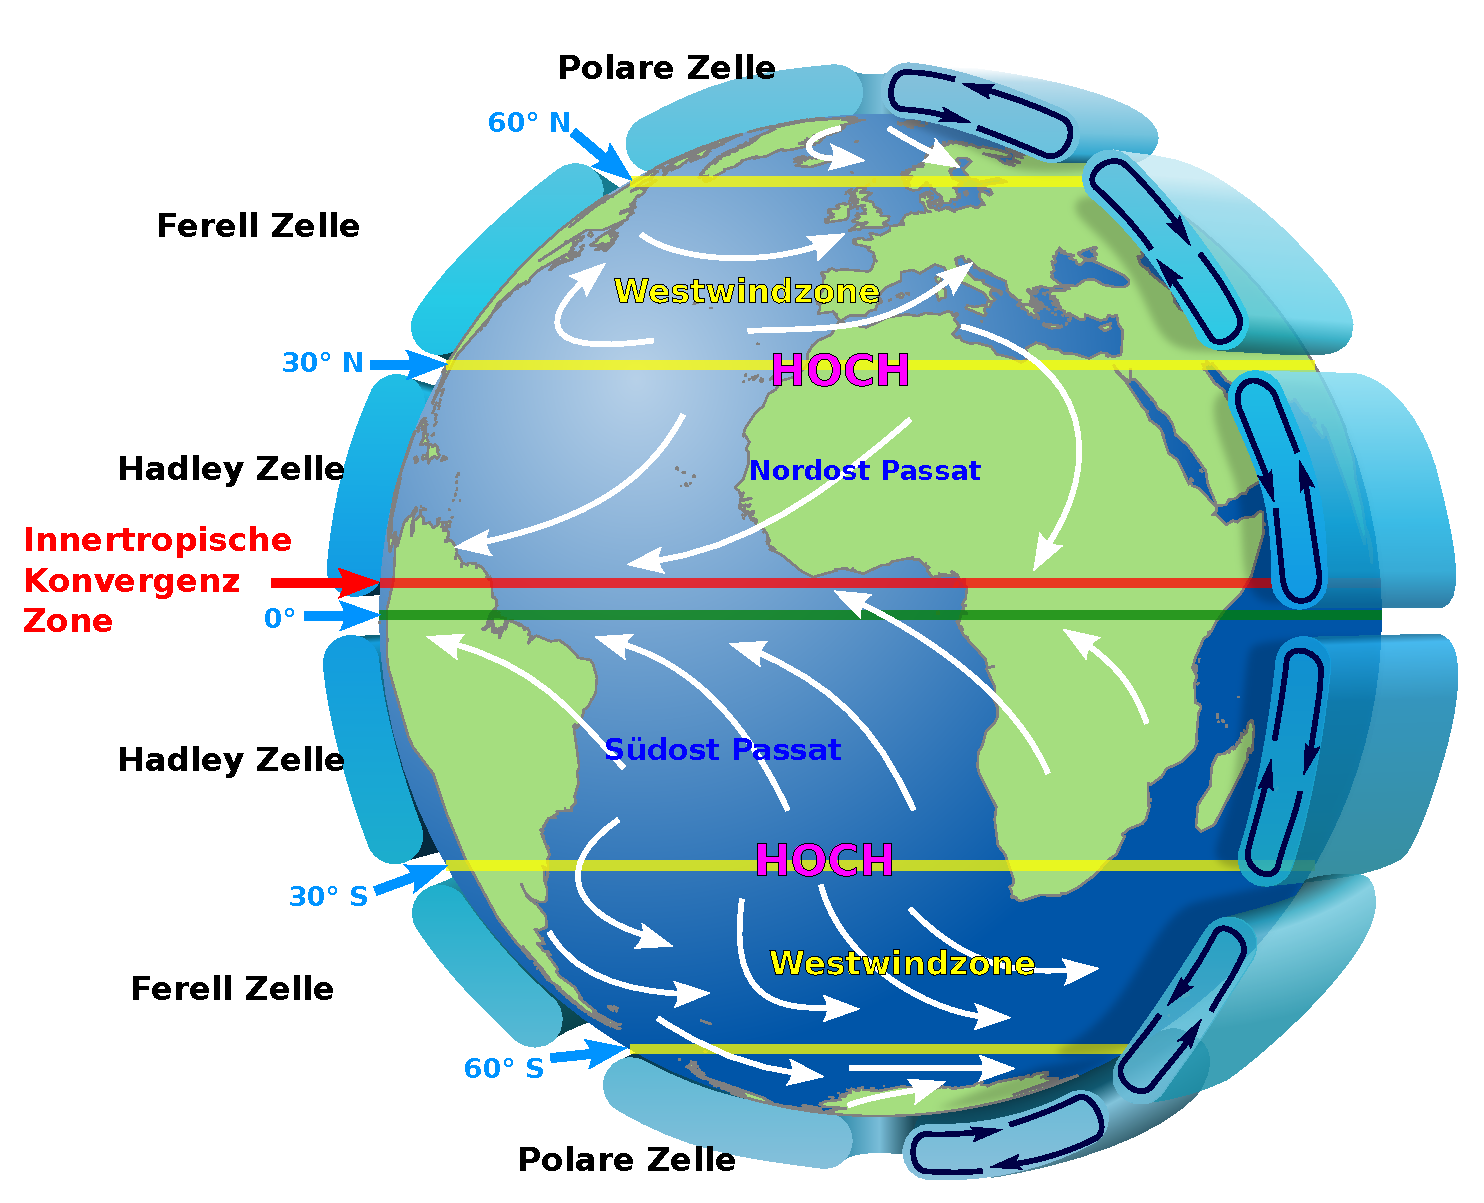
\includegraphics[width=.65\linewidth]{bilder/Earth_Global_Circulation_-_de.pdf}
		\caption{Globale atmosphärische Zirkulation, Quelle: MireRun/Kaidor nach NASA Global circulation of Earth's atmosphere}
	\end{figure}

	\note{
	Großskalige Modellvorstellung globaler Zirkulationssysteme in der Atmosphäre

	Starke Vereinfachung:
		\begin{itemize}
			\item[] Am Äquator steigt warme Luft auf, hinterlässt ein Tiefdruckgebiet (weniger Luft vorhanden).
    	\item[] In Bodennähe strömt kältere Luft in Richtung Äquator nach.
			\item[] Wegen der Drehung der Erde (Corioliskraft) werden Bewegungen auf der Nordhalbkugel im Uhrzeigersinn abgelenkt, auf der Südhalbkugel gegen den Uhrzeigersinn. Eine äquatorwärts strömende Luftmasse wird dadurch auf der Nordhalbkugel zum Nordostwind, auf der Südhalbkugel zum Südostwind.
			\item[] In der Höhe kommt es zu Ausgleichsströmungen: Luftmassen, die über dem Äquator aufgestiegen sind, strömen in der Höhe wieder polwärts. Am Pol in der Höhe eintreffende Luftmassen sinken dort ab.
		\end{itemize}

		Etwas genauer:
		\begin{itemize}
			\item[] vom Äquator weg strömende Luftmassen, sinken wegen der polwärtigen Flächenkonvergenz der Erde über rund \SI{30}{\degree} Breite wieder ab (Hadley Zelle, Passatwinde).
			\item[] vom Pol weg strömende Luftmassen, erwärmen sich, steigen ab rund \SI{60}{\degree} Breite wieder auf (Polare Zelle).
    	\item[] Zwischen beiden Systemen jeder Hemisphäre jeweils ein dritte, gegenläufige Zelle (Ferell Zelle, Westwinde).
    	\item[$\rightarrow$] Sowohl auf der Nord- als auch auf der Südhalbkugel jeweils drei (bodennahe) Windsysteme,
			\item[] Innertropische Konvergenzzone trennt Nord- und Südhalbkugel, Tiefdruckrinne
		\end{itemize}
		\begin{itemize}
			\item[Hadley Z.] Passatwinde sehr stabil, zur schnellen Überquerung der Ozeane genutzt
			\item[Polare Z.] Sehr stabil
			\item[Ferell Z.] instabil, gegenläufig zu polarer Zelle und Hadley Zelle. Enthält ca. \SI{38}{\percent} der Energieunterschiede zwischen Pol und Äquator.
		\end{itemize}
	}
\end{frame}
